% %%%%%%%%%%%%%%%%%%%%%%%%%%%%%%%%%%%%%%%%%%%%%%%%%%%%%%%%%%%%
\section*{Results}
% %%%%%%%%%%%%%%%%%%%%%%%%%%%%%%%%%%%%%%%%%%%%%%%%%%%%%%%%%%%%

We developed a real-time closed-loop optogenetic system to regulate population activity within a targeted cortical region, monitored using wide-field calcium imaging. Trial-averaged cortical responses to optogenetic stimulation obeyed a stationary linear input--output map, providing the empirical foundation for controller design.

% ------------------------------------------------------------
\subsection*{Experimental setup and closed-loop control architecture}
% ------------------------------------------------------------ 
The closed-loop experiments were performed in head-fixed transgenic GCaMP and opsin-expressing mice in a behavioral chamber \citep{Matveev2024}. The front limbs of the mice rested on a freely moving wheel, and a blank screen was present in front of the mouse.
Neural activity was recorded at 35\,Hz using wide-field calcium imaging (Fig.~\ref{fig:figure1}A), and spatially resolved optogenetic stimulation was applied to a targeted cortical region neighboring the $\Delta F/F$ output zone as depicted in Fig.~\ref{fig:figure1}B. The stimulation region was picked to be close to the output kernel (Fig.~\ref{fig:figure1}C) so as to directly inhibit the region's activity.
We then designed a hardware and software architecture for signal processing and fast closed-loop control of this mesoscale activity (Fig.~\ref{fig:figure1}D). The software layer handled the mathematical framework required for computing control signal through feedback.
We designed a proportional--integral (PI) feedback controller with open-loop compensation to drive cortical activity toward the reference $\Delta F/F$ value(Fig.~\ref{fig:figure1}E).
The open-loop component provided the nominal stimulus required to reach a reference state based on the calibrated controller gains, while the PI feedback component added real-time error correction to compensate for bias due to inaccurate open loop gains, residual nonlinearities, and spontaneous trial-to-trial fluctuations.
The control system as depicted in Fig.~\ref{fig:figure1}E, treats the kernel averaged wide-field measurements as outputs, the controller uses the error between output and reference signal to compute an optogenetic stimulus input to the plant, subject to a processing and physiological delay that closes the loop (Fig.~\ref{fig:figure1}F). The system has an inherent maximum latency of 47\,ms, computed as the time between signal arrival at the cortical level and application of the laser.

\begin{figure}[h]
    \centering
    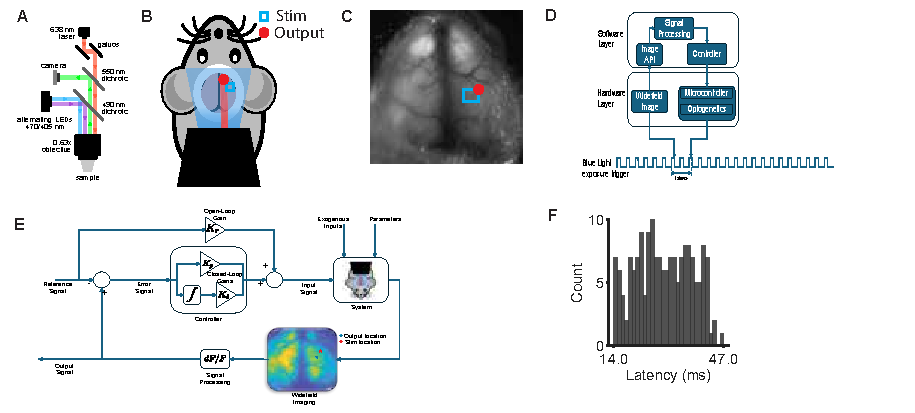
\includegraphics[width = \linewidth]{images/Figure1.pdf}
    \caption{Experimental setup and closed-loop control architecture.\\
    \small{
    \textbf{A:} Schematic of the widefield microscope optical path. Blue (470\,nm) and violet (405\,nm) LEDs illuminate the dorsal cortex; emitted green photons are collected by the camera via two dichroics. A red (638\,nm) galvanometer-steered laser passes through both dichroics to deliver spatially targeted optogenetic stimulation.\\
    \textbf{B:} Dorsal cortex schematic showing the spatial relationship between the optogenetic stimulation target (red) and the $\Delta F/F$ output region (blue box).\\
    \textbf{C:} Representative widefield frame showing the stimulation spot (red) and the spatial kernel used as the closed-loop feedback output (blue box).\\
    \textbf{D:} Signal-flow diagram of the closed-loop pipeline. A hardware trigger initiates frame acquisition; the image API streams frames to the control server, which computes $\Delta F/F$ and evaluates the controller; the resulting command drives the optogenetic stimulator via a microcontroller.\\
    \textbf{E:} Block diagram of the closed-loop control architecture. The spatial-kernel $\Delta F/F$ average provides the output $y_t$; the PI controller computes a corrective input from the tracking error and sums it with the feedforward term; the combined signal drives the laser, subject to an end-to-end latency of 80\,ms.\\
    \textbf{F:} Distribution of measured end-to-end control-loop latencies across all sessions (3 mice, 13 sessions). Latency is defined as the time from camera trigger to laser activation command, encompassing image transfer, $\Delta F/F$ computation, and digital-to-analog conversion.
    }}
    \label{fig:figure1}
\end{figure}

% ------------------------------------------------------------
\subsection*{Trial-averaged cortical dynamics are approximated by a linear system}
% ------------------------------------------------------------
Trial-averaged cortical responses followed a linear input--output map for impulse based stimulation, and a linear dynamical system closely approximated impulse and step responses for cortical stimulation using optogenetics. 
We delivered optogenetic impulse inputs at discrete amplitudes between 0--1.8\,mW powers, randomly interleaved across trials for each session. The Fig.~\ref{fig:figure2}A, shows the trial averages impulse response for one of the experiment sessions, which is used to characterize settling time($\sim200$ms) for impulse response.
We found that the mean of the distribution of total inhibition energy(see Methods) per trial, had a monotonic relationship with stimulation amplitudes, therefore it could be approximated with a linear relationship across the three sessions (Fig.~\ref{fig:figure2}B; $R^{2} = 0.99, 0.51, 0.94$; slope $= -0.36, -0.57, -0.58$). This linear relationship between stimulation amplitude and inhibition energy supports the design of an open-loop controller calibrated from impulse response data that relies on monotonicity of the input output relationship~\citep{astrom1995pid}.

\begin{figure}
    \centering
    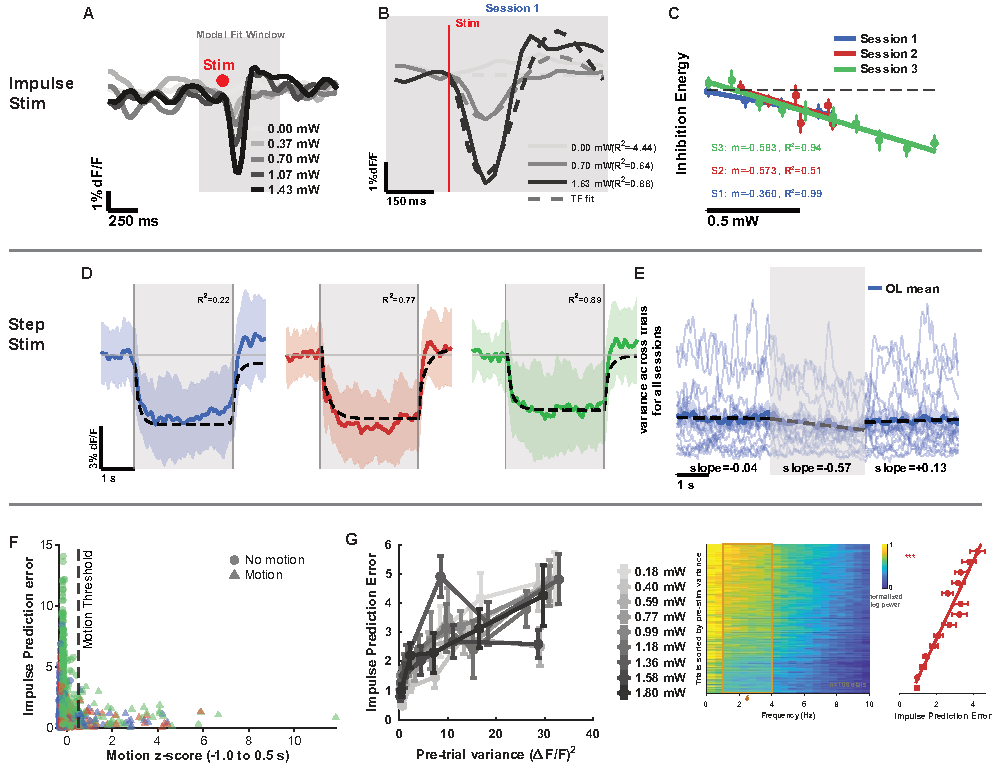
\includegraphics[width = \linewidth]{images/Figure2_extra.pdf}
    \caption{Input-output characterization of local cortical dynamics.\\
    \small{
    \textbf{A:} Trial-averaged $\Delta F/F$ impulse responses across five stimulation amplitudes (0--2.7\,V; $\sim$90 trials per amplitude). Traces are aligned to stimulation onset (red line); shading shows $\pm$1\,SD across trials. Amplitude was randomly sampled on each trial.\\
    \textbf{B:} Inhibition energy denoting the total suppression for 0-200ms versus stimulation amplitudes for three sessions. Points show mean $\pm$ SD across trials ($\sim$50 trials per amplitude); lines show the fitted linear input-output relationship (see Methods). $R^{2} = 0.94, 0.51, 0.99$ across three sessions.\\
    \textbf{C:} Prediction of trial-averaged traces of three representative impulse responses. The bold traces show the trial-averaged response and the dashed responses show LTI system fit to the trial averaged data($N = 90 $trials).
    \textbf{D:} Prediction of trial-averaged traces of three representative step responses. The bold traces show the trial-averaged response and the dashed responses show LTI system fit to the trial averaged data($N = 50 $trials).
    \textbf{E:} Traces showing variance across trials for an experiment session. We show variance traces for 13 session across stimulation window(gray) of three seconds, along with 3 second pre and post stim windows. The bold trace shows average of all variance traces. The dashed lines show the linear approximation of the average variance trace, the slope of this line is shown for the pre, during, and post sti windows.}}
    \label{fig:figure2}
\end{figure}

Step inputs applied over 3-second trial windows produced trial-averaged trajectories that were closely approximated by a LTI system. We fit LTI systems to trial-averaged, step response data from three different sessions as shown in Fig.~\ref{fig:figure2}D. The LTI system was fit to learn step response of a low dimensional transfer function 
consistent with marginally stable oscillatory dynamics in biologically bounded cortical circuits. 
Open-loop stimulation modestly reduced across-trial variance during stimulation (post-onset slope $-0.57 \pm 0.24$\,($\Delta F/F$)$^2$/s, vs.\ near-zero pre-onset slope $-0.04 \pm 0.14$, $n=13$ sessions); closed-loop feedback produced a further and more consistent reduction. Under open-loop step stimulation, trial-to-trial variance did not change around stimulus onset (Fig.~\ref{fig:figure2}C), indicating that optogenetic input did not destabilize the system.
Session-to-session offset bias in the step response informed inclusion of the integral term in the PI controller (see Materials and Methods).
Batch-mean $\Delta F/F$ variance during spontaneous activity decreased monotonically with trial count, stabilizing beyond approximately 50 trials per session (Fig.~\ref{fig:S1}), consistent with the trial-averaging assumption (see Materials and Methods). \todo{Also verify that the batch mean itself stabilizes across batch sizes — variance convergence (CLT) holds for any finite-variance process including drifting ones, and does not alone establish zero-mean disturbances.}
Convergence rates differed across sessions recorded from the same region, consistent with session-to-session differences in brain state.

% ------------------------------------------------------------
\subsection*{Closed-loop control improves reference tracking accuracy}
% ------------------------------------------------------------

Across sessions in \todo{INCONSISTENCY: this says ``two mice'' but Fig.~3 caption says ``3 mice, 13 sessions'' and Fig.~1F caption also says ``3 mice, 13 sessions''. Determine the correct mouse count (AL\_0033 + AL\_0039 = 2 mice, but total sessions = 13 spans additional animals?) and apply consistently throughout.} two mice with confirmed opsin expression, closed-loop feedback consistently improved tracking of $y_{\mathrm{ref}} = -5\%\,\Delta F/F$ relative to open-loop stimulation (Fig.~\ref{fig:figure3}A--D). 
Under open-loop conditions, the feedforward term produced cortical responses that systematically deviated from the reference, reflecting the inability of a fixed input to compensate for ongoing spontaneous fluctuations or inaccuracies in the estimated gain $K_{r}$.
Under closed-loop control, the proportional term corrected instantaneous deviations while the integral term accumulated and eliminated persistent offset, yielding substantially improved alignment with $y_{\mathrm{ref}}$ at the single-trial level (Fig.~\ref{fig:figure3}A).


\begin{figure}
    \centering
    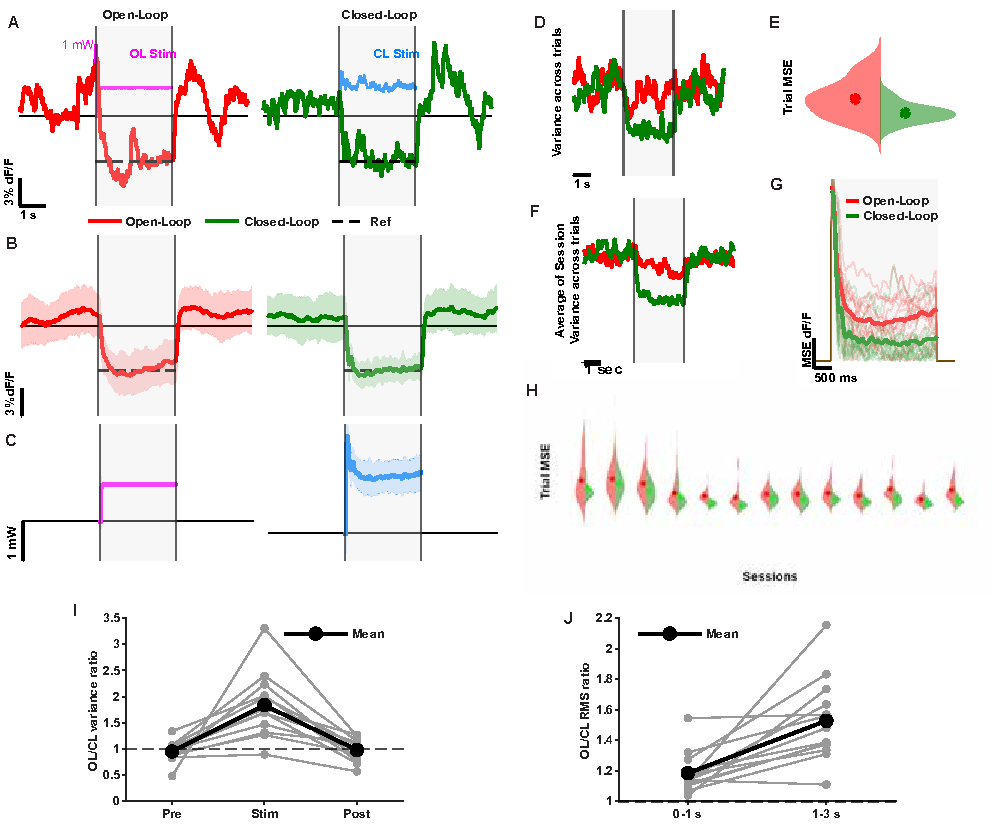
\includegraphics[width = \linewidth]{images/Figure3_extra.pdf}
    \caption{Closed-loop versus open-loop cortical activity control (2 mice, 13 sessions).\\
    \small{
    \textbf{A:} Single-trial example of open-loop (red) and closed-loop (green) $\Delta F/F$ responses. Gray shading marks the 3\,s stimulation window; dashed line indicates the target $-5\%\,\Delta F/F$. Bottom traces show the corresponding optogenetic input signals.\\
    \textbf{B:} Trial-averaged $\Delta F/F$ responses under open-loop (red) and closed-loop (green) control for a representative session. Bold lines show the trial mean; thin lines show individual trials.\\
    \textbf{C:} Trial-averaged optogenetic input signals for open-loop (pink) and closed-loop (blue) conditions. Bold lines show the mean input; thin lines show individual trials.\\
    \textbf{D:} Cross-trial variance of $\Delta F/F$ as a function of time for open-loop and closed-loop conditions, for a representative session. Gray shading marks the stimulation window.\\
    \textbf{E:} Distribution of per-trial tracking MSE (mean squared error over the 3\,s stimulation window) for open-loop and closed-loop conditions, shown as violin plots. Points indicate individual trials.\\
    \textbf{F:} Cross-trial variance during the stimulation window, averaged across all 13 sessions, for open-loop and closed-loop conditions.\\
    \textbf{G:} Per-trial MSE distributions pooled across all 13 sessions, shown as violin plots.\\
    \textbf{H:} Mean absolute tracking error per unit time as a function of time within the trial, averaged across all sessions (bold) with individual session traces (thin lines).\\
    \textbf{I:} Ratio of variance across trials for OL and CL trials for each session, for pre-stim window(stim-start $- 3$sec to stim), stim window and post stim (stim-end to stim-end $+3$ seconds) window. The gray lines depict individual sessions and bold line represents mean of all sessions.\\
    \textbf{J:} Controller disturbance rejection effect shown by splitting trial into $0-1$sec and $1-3$sec regimes depicting setting time and stable activity regimes, the y-axis show ratio of OL and CL tracking error RMS for each experiment session. The gray lines depict individual sessions and bold line represents mean of all sessions.
    }}
    \label{fig:figure3}
\end{figure}

Trial-averaged responses confirmed that closed-loop activity followed the reference closely throughout the stimulation window, whereas open-loop responses exhibited systematic positive bias (Fig.~\ref{fig:figure3}B).
The difference in average input responses between conditions (Fig.~\ref{fig:figure3}C) reflects the additional corrective signal contributed by real-time feedback. 
Per-trial tracking costs shifted toward lower values and showed reduced spread under closed-loop control (Fig.~\ref{fig:figure3}E), indicating both improved mean performance and enhanced reliability of neural modulation across trials. \todo{Re-compute per-trial MSE over t = +1 s to +3 s post-laser onset; update figures and text once recomputed (see MEETINGS.md 2026-05-08).}
These improvements held across all recorded sessions (Fig.~\ref{fig:figure3}G) and required small controller gains. For the session shown in Fig~\ref{fig:figure3}A-E we used the gains, $K_{r} = \mathbf{0.1}, K_{p} = \mathbf{0.07} \& K_{i} = \mathbf{0.1}$, suggesting that the approximately linear, stationary input--output structure identified empirically was sufficient to support stable PI feedback.

% ------------------------------------------------------------
\subsection*{Brain states affects predictability}
% ------------------------------------------------------------

\todo{SECTION INCOMPLETE — write the pre-stimulus brain state paragraph here. Key result (FINDINGS.md, prestim\_variance.m): OL regression slope of pre-stim variance vs.\ per-trial MSE is positive (higher pre-stim variance $\to$ higher error); CL slope is near-flat, indicating feedback decouples performance from initial brain state. Add K2 figure reference. Also implement Curto \& Issa-style trial-sorting figure: split trials by $\sim$1\,s pre-stim variance (synced vs.\ desynced); sort within groups by $|\Delta F/F|$ at $t=0$; display heatmaps for OL and CL. Verify authorship: Curto, Bhatt \& Issa (2009) before citing. Consider 500\,ms or sliding window instead of 1\,s (may conflate state transitions, per MEETINGS 2026-05-11).}

% ------------------------------------------------------------
\subsection*{Closed-loop control reduces trial-to-trial variability}
% ------------------------------------------------------------
In addition to improving mean tracking accuracy, closed-loop feedback substantially reduced trial-to-trial variability in cortical activity during the stimulation window (Fig.~\ref{fig:figure3}D--F). 
This result follows from the structure of the PI controller: individual trial trajectories are perturbations of the nominal averaged response driven by zero-mean neural disturbances and trial-to-trial brain-state fluctuations, and the controller actively steers each trial back toward the reference, compressing the cross-trial distribution of responses.

\todo{INCONSISTENT WITH FINDINGS: ``remained largely unchanged'' contradicts the variance claim fix needed at the sentence above (post-onset OL slope $= -0.57 \pm 0.24$ is not ``unchanged''). Once the variance sentence in the previous section is rewritten, update this sentence to match — likely: ``Under open-loop stimulation, variance modestly decreased relative to the pre-stimulation baseline\ldots''} During open-loop stimulation, response variance remained largely unchanged relative to the pre-stimulation baseline, reflecting the inability of the fixed feedforward term to counteract spontaneous fluctuations. Under closed-loop control, variance decreased substantially during the stimulation window, consistent with active disturbance rejection. This reduction persisted across sessions, as confirmed by pooled within-session variance traces (Fig.~\ref{fig:figure3}D--F) and by the cross-session distribution of per-trial MSE (Fig.~\ref{fig:figure3}G).

The validity of these results depends on the trial-averaging assumption holding across the session. The empirical variance convergence in Fig.~\ref{fig:S1} supports this assumption over the 100-trial validation period. 
Performance varied across animals and sessions, likely reflecting residual non-stationarity in arousal and behavioral state, differences in opsin expression, and session-to-session variation in the spatial overlap between stimulation and output regions.
Despite this variability, directional improvements in both tracking accuracy and trial-to-trial variance were consistent across all experiments.


We observed that motion affected trials 
\todo{PLACEHOLDER — Curto \& Issa-style trial-sorting figure (see MEETINGS.md 2026-05-11). Split trials into synchronized (high pre-stim variance, $\sim$1\,s window) vs.\ desynchronized (low pre-stim variance). Within each group, sort trials by absolute fluorescence at $t = 0$. Display $\Delta F/F$ heatmaps for CL and OL conditions. Verify authorship before citing: Curto, Bhatt, Issa (2009). Note: 1\,s pre-stim window may conflate state transitions — consider 500\,ms or sliding window.}

% ------------------------------------------------------------
\subsection*{Disturbance attribution: spectral and motion analysis}
% ------------------------------------------------------------
\todo{PLACEHOLDER — Confirm absolute power spectra (ΔF/F$^2$/Hz) complete; finalize narrative framing (motion + frequency → trial outcome). Determine what fraction of high-error CL trials are attributable to 2--4\,Hz spontaneous fluctuations vs.\ motion. Add motion vs.\ MSE (CL vs.\ OL, cross-session) scatter panel and good/bad trial spectral examples to manuscript (see MEETINGS.md 2026-05-11).}

% ------------------------------------------------------------
\subsection*{Contralateral cortex predicts ipsilateral activity}
% ------------------------------------------------------------
\todo{PLACEHOLDER — Three-layer contralateral-prediction model figure (see MEETINGS.md 2026-05-11). Pink: predict ipsilateral ROI from contralateral pixels in spontaneous (no-opto) data. Orange: add average OL impulse response on top. Red: add per-trial laser sequence via TF model; validate against CL traces. Add motion energy as co-predictor. If red model validates: compute post-hoc optimal laser sequence for representative trials, quantify gap vs.\ actual controller, frame as MPC motivation.}

% ------------------------------------------------------------
\subsection*{Feedforward and preview control}
% ------------------------------------------------------------
\todo{PLACEHOLDER — Feedforward (sine-wave) and preview control results (deferred since 2026-04-27; see PAPER.md). Add plots for variable sine-wave reference. Classify feedforward vs.\ preview control. Compare against naive CL baseline. Requires new section in manuscript with literature context.}
